%!TEX root = ../main.tex
% -*- root: ../main.tex -*-
\section{Implementation}\label{sec:implementation}


To demonstrate the feasibility of our model
in managing the life-cycle of continuum applications, in this paper we also present working prototypes of for the domain manager and mobile middleware implementing A3-E. In particular, the former consist of a mobile domain and a local-edge domain managers, while the latter consists of a mobile middleware for Android platform devices. Later on, these prototypes are employed in the evaluation of our model.

In this paper we rely on existing FaaS platforms~\cite{AWSLambda, OpenWhisk} for handling the Allocation of $\mu$-services to a pool of dynamically allocated containers. A more sophisticated approach based on control-theory~\cite{Quatrocchi2016discrete} is considered future work (see Section~\ref{sec:conclusions} for more details).

%dedicated to the domain-side dynamic resource provisioning is considered future work;

%more precisely we will use lightweight control theoretical planners that were recently proved to be well-suited to control containerized applications~\cite{Quatrocchi2016discrete} (see Section~\ref{sec:conclusions} for more details).

%To demonstrate the feasibility of our model
%in managing the life-cycle of continuum applications
%, we describe an implementation of A3-E. Due to its complexness, in this section we focus on the self-management loops handling Allocation from both provider and client viewpoints. %Nonetheless, a complete prototype was used for the evaluation in Sec.~\ref{sec:evaluation}.

\subsubsection{Domain-side Middleware}










%Martin's old server side details

%Figure~\ref{fig:reference-architecture} shows the proposed architecture for the compute continuum. Particular focus is put on the interaction between devices and Edge domain servers, since it is the main contribution of this paper. 
%The main physical elements are mobile devices and domain servers. Mobile devices can be of any type (e.g., tablets, smartphones), running several low-latency applications that needs offloading part of their computation to more powerful servers. For this, the devices send information to be processed to the domain server through standardized network protocols~\cite{Sill17standards}.  A Base Transceiver Station\footnote{Different generations of wireless mobile networks use distinct names (e.g., eNodeB in 4G).} (BTS) bridges mobile devices and domain servers as a part of the cellular infrastructure and  Edge architecture, according to its current specifications~\cite{hu2015mobile}. In this scenario, mobile devices and Edge domain servers are at no more than a few hops from each other. These servers host a serverless infrastructure, where stateless functions are deployed and executed according to the phases defined by the A3-E model. 
%The following sections provide details about the A3-E middleware (Section~\ref{subsec:A3-E}) and the serverless infrastructure that materializes Edge domain servers (Section~\ref{subsec:ServerlessArchCont}).
%
%\subsection{Edge-FaaS}
%\label{subsec:ServerlessArchCont}
%
%Following we briefly describe the serverless architecture that materializes the notion of Edge domains --- as shown in Figure~\ref{fig:domain-edge-arch}. 
%
%\begin{figure}[htb]
%	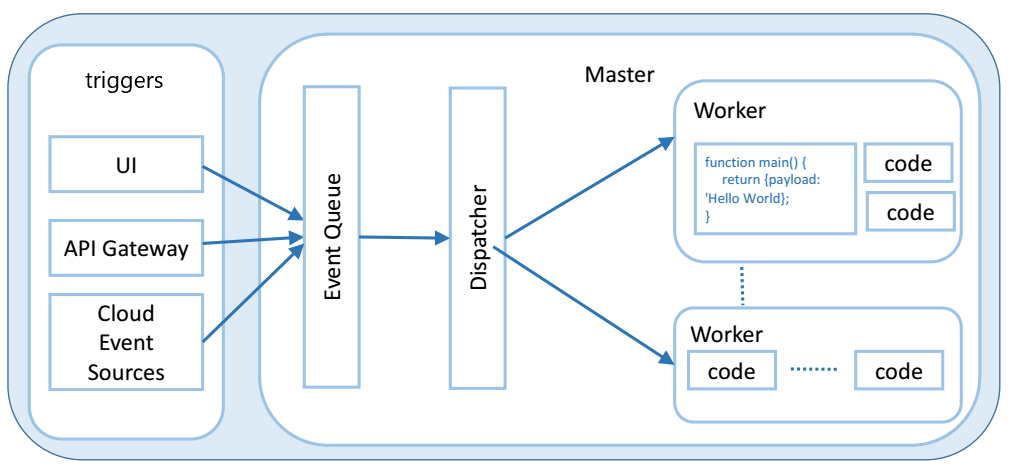
\includegraphics[width=.7\textwidth]{figs/ServerlessGenericArchEdit}
%	\caption{Serverless Architecture in the Domain Server}
%	\label{fig:domain-edge-arch}
%\end{figure}
%
%While Edge servers are ideal candidates for offloading the computation to preserve devices' battery life and reduce latency, these domain nodes are themselves potentially resource-constrained. Accordingly, the feasibility of hosting dedicated \textit{virtual machines}, \textit{containers}, and \textit{stateful applications} would also be limited, as these nodes cannot scale ``infinitely" to host always-running VMs/containers as the cloud itself. To overcome this limitation, we propose to materialize Edge domain servers through a serverless architecture~\cite{Roberts:2016,GarrigaMendonca2017}. 
%
%Figure~\ref{fig:domain-edge-arch} details the serverless components deployed on the domain server. The entry points are the \textit{triggers} associated with events --- e.g.,  mobile sensor readings or HTTP requests from mobile apps.  
%%in the MAR application, an event that triggers a function consists of uploading of an image or capturing a frame with the device's camera. --e.g., changes to database records, mobile sensor readings, code commits to a repository, or simple HTTP requests from Web or mobile apps. 
%These triggers fire requests to an \textit{Http Server} that exposes available functions as REST endpoints. 
%
%To achieve network transparency, a local Domain Name Server (DNS), deployed on the cellular infrastructure, must distinguish between requests addressed to the A3-E middleware/RESTful functions exposed by the domain server, and any other request for an Internet endpoint. The main difference from a regular DNS is locality, as the requests must be handled by the domain server on the current base station. To this end, the names of edge resources must be resolved locally without being propagated to public DNS servers. Whereas the specific details of the naming solution are outside the scope of this work, we argue that such a feature should not pose a significant technical challenge.% as it is already partially supported by the cellular infrastructure [CITE? is it right?].
%
%Once a request reaches the domain server, it is then forwarded to a \textit{controller} component, which identifies and retrieves the function being called, authorizes the execution of such a function and identifies an available invoker to run it. \textit{Invokers} isolate the \textit{functions} in containerized environments, optimized and managed by the serverless provider to reduce overhead and response time. Note that cold starts can happen when the controller allocates an inactive/new function for the first time. It increases time for the first call while the provider provisions the invoker (runtime container) and then runs the function. However, when the function is still allocated or warm --- since it was engaged recently by the same or a different client --- the environment stays alive, ready and waiting for execution. Eventually, after a period of inactivity (that depends on the size of the function and the current load of the server), the provider can drop the container and the function be deallocated, freeing resources for other functions.
%
%
%Finally, after execution, results and logging information are stored in the \textit{Storage} component, a highly available, noSQL database. Note that most of the components of the serverless architecture of the domain server are shared 
%%(in grey in Figure~\ref{fig:abstract_architecture}) 
%among all the functions. The highly shared nature and the automated management of the whole platform allows any function allocated on the domain servers to scale up automatically and elastically to unexpected bursts in the workload, and to scale down when it is not used anymore. In contrast with container-based stateful applications, the serverless platform is responsible for allocating functions of one or more applications on a pool of shared containers, according to the resources available at the domain server. As a result, the use of the computational resources of domain servers is optimized, allowing both more functions to be deployed and more requests to be processed simultaneously.
%
%Needless to say, an IaaS/FaaS cloud domain can always be selected to allocate and engage functions when required --- due to unavailability/overload of edge domain servers. Their implementation is similar to those described above, although details can vary among different vendors\footnote{\url{https://github.com/apache/incubator-openwhisk/blob/master/docs/about.md}}.
%
%As an advantage over the traditional, ``serverful'' approaches, it is not necessary to pre-allocate multiple virtual machines or containers to be resilient and responsive against downtime of single instances or bursts of workload. The on-demand execution of functions provides inherent scalability and optimal utilization as the number of running functions always matches the trigger rate. Additionally, the application developer only focuses on the application code and can fully outsource the management of the execution infrastructure to the A3-E middleware. The serverless approach also provides a fine-grained \textit{pay-per-use} billing model with benefits for both application owners and telecom operators (in charge of the domain servers).

\subsection{Mobile Middleware}~\label{sec:mobile_middleware}

%\begin{figure}[tbp]
%	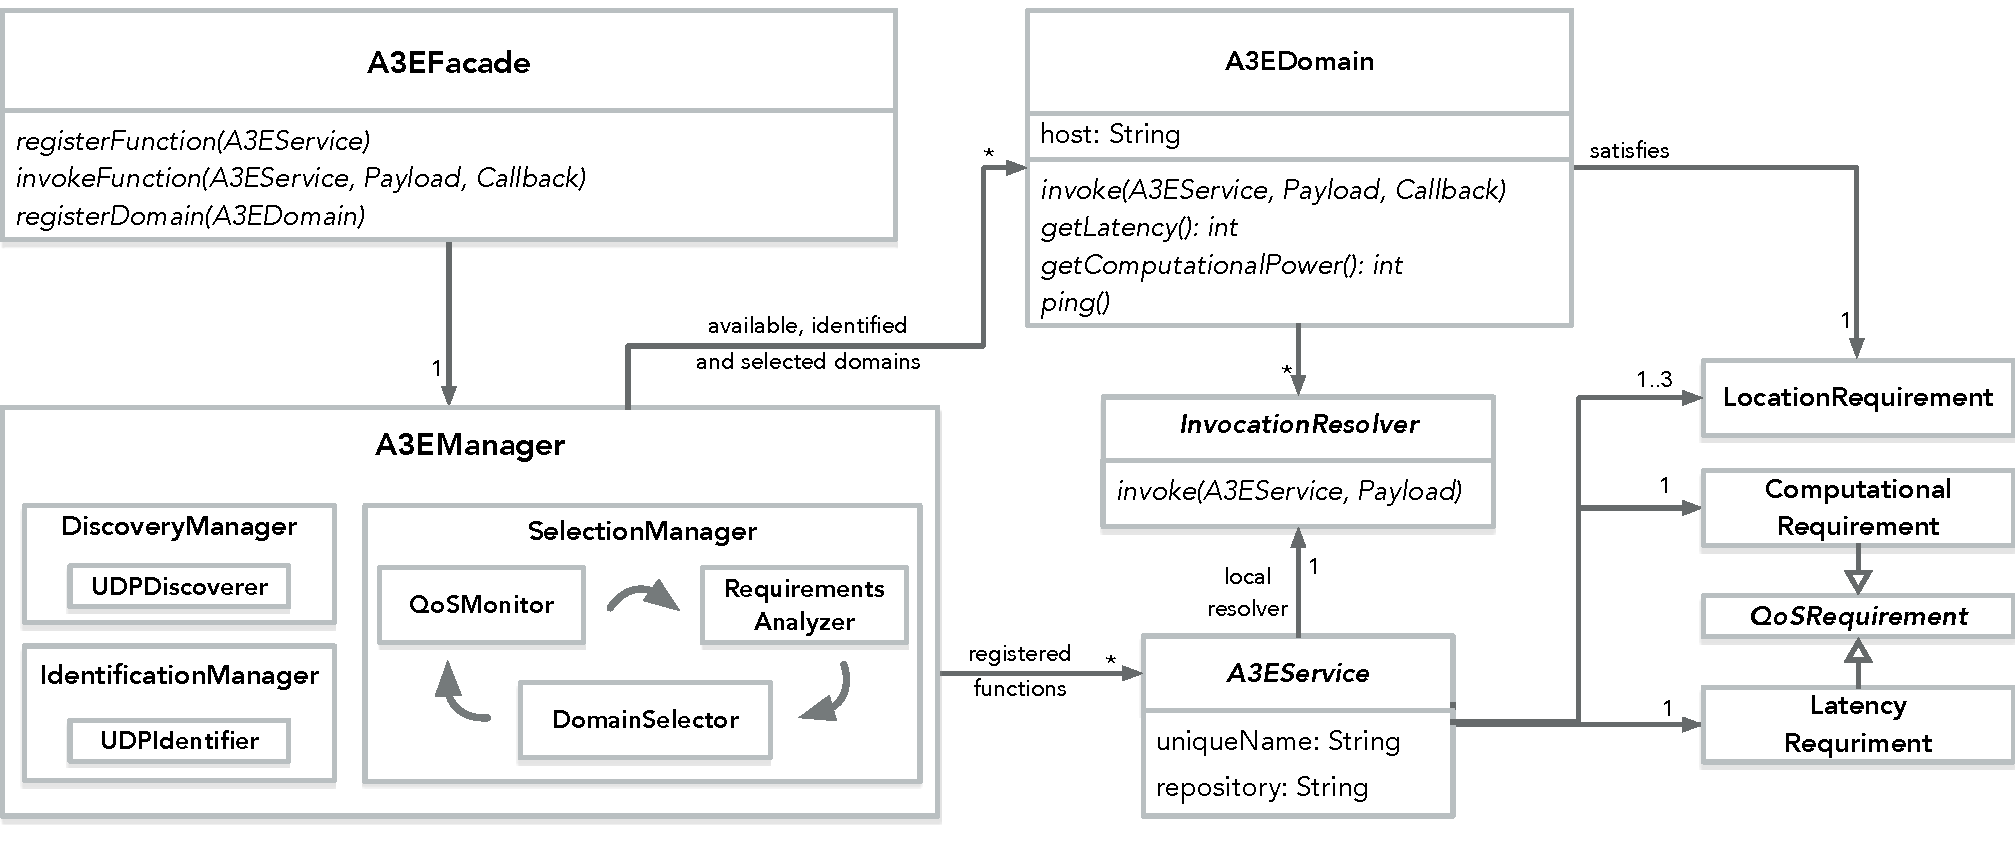
\includegraphics[width=1\textwidth]{figs/a3e-mobile-prototype}
%	\caption{Client-side Middleware Architecture}
%	\label{fig:mobile-prototype}
%\end{figure}

%TODO [Danilo] consider moving part of this nice introduction to the formulation (Sec. 2.3)
The main goal of the client-side middleware~\footnote{Documentation and source code are available at \url{https://github.com/deib-polimi/A3-E-CSM}} is to allow client applications to invoke A3-E microservices without knowing where they will actually be executed within the computing continuum: locally on the mobile domain, in a local-edge server, in a mobile-edge server, or in the cloud. Its selection algorithm is a multi-objective function that takes into account the measured QoS and the requirements. The provided implementation targets Android-based devices. However, it does not use Android-specific technology and can therefore be generalized to other mobile platforms. 

To implement Awareness, the middleware listens for \textit{domain identification} signals sent by its mobile domain and broadcasted by edge domains. To avoid battery drain, edge domains discovery happens for a short period after the mobile middleware is first executed or the device's network state changes (e.g., from a local-area Wi-Fi to a cellular network). 

For every domain found, the middleware proceeds with Acquisition by sending a \textit{client identification} signal containing a Git repository from which $\mu$-service function(s) and dependencies can be downloaded, in case of edge domains; or the qualified name of function(s), in case of the mobile domain. Finally, as in this paper cloud domains have been evaluated with an existing FaaS platform lacking A3-E's Awareness and Acquisition, cloud domains are acquired programmatically.


%Further optimization could be achieved by employing state-of-art advertisement and discovery approaches. 

The mobile middleware implements A3-E's Allocation as a self-managing loop that: (i) monitors $\mu$-services provided by different domains in terms of QoS metrics; (ii) analyzes the best alternative satisfying requirements of the client application; and (iii) updates the domain selection for a given $\mu$-service. In specific, the analysis consists of a multi-attribute rating that takes into account the measured QoS attributes and application requirements.

%TODO [Danilo] make sure we introduce requirements before or add the missing bullet below 
%In addition to A3-E's \textit{Location requirements}, 
The prototype considered three types of $\mu$-service requirements: a \textit{Location Requirement} constrains where the $\mu$-service can be placed within the continuum, i.e., \textit{LOCAL}, \textit{LOCAL\_EDGE}, \textit{MOBILE\_EDGE}, or \textit{CLOUD} or a combination of the above;  a \textit{Latency Requirement} constrains network latency, i.e., \textit{ANY}, \textit{LOW} or \textit{VERY\_LOW}; and a \textit{Computational Requirement} defines how relevant it is for a $\mu$-servi to have fast computing, i.e., \textit{ANY}, \textit{FAST} or \textit{VERY\_ FAST}. 

%{\small
%\begin{enumerate}
%	
%	\item a \textit{Location Requirement} constrain where the $\mu$-service can be placed within the continuum, i.e., \textit{LOCAL}, \textit{LOCAL\_EDGE}, \textit{MOBILE\_EDGE}, or \textit{CLOUD} or a combination of the above; 
%	
%	\item a \textit{Latency Requirement} constrains network latency, i.e., \textit{ANY}, \textit{LOW} or \textit{VERY\_LOW}; and 
%	
%	\item a \textit{Computational Requirement} defines how relevant it is for a $\mu$-servi to have fast computing, i.e., \textit{ANY}, \textit{FAST} or \textit{VERY\_ FAST}. 
%\end{enumerate}
%}%

Computational requirements defined as a fixed score ranging from $1$ to $5$\footnote{Labeling computational power is also common in the cloud where different tiers of virtual machines are available -- \url{https://aws.amazon.com/ec2/instance-types/}}. By default, the mobile domain has a score of $1$, edge domains have a score of $4$, while cloud domains have a score of $5$. As cloud provides the illusion of infinite scalability it gets the maximum score, regardless of the VMs that are actually being used. 

%with dynamic scores taking into account the saturation of the domain or the device's battery level (in the case of a mobile domain).
\setlength{\textfloatsep}{5pt}% Remove \textfloatsep
{\scriptsize
\begin{algorithm}[h]
	\caption{A3E Selection Algorithm}
	\label{alg:selection}
	\begin{algorithmic}[1]		
		\Function{selectDomain}{A3EService service, A3EDomain[] $identifiedDomains$}
		\State$scoreRange \gets 5$
		\State $maxLatency \gets \Call{computeMaximumLatency}{identifiedDomains}$
		\State $maxCpuPower \gets \Call{computeMaximumComputationalPower}{identifiedDomains}$
		\State $latencyWeight \gets service.getLatencyRequirement()$ 
		\State $cpuPowerWeight \gets service.getComputationalPowerRequirement()$ 
		\State $maxScore \gets 0$
		\State $selectedDomain \gets null$
		\ForAll{$domain \in identifiedDomains$ } 
		\State $latency \gets domain.getLatency()$ 
		\State $cpuPower \gets service.getComputationalPower()$ 
		\State $latencyScore \gets latencyWeight*((scoreRange-1)*(1 - latency/maxLatency)+1)$ 
		\State $cpuPowerScore \gets cpuPowerWeight*(scoreRange*(cpuPower/maxCpuPower))$
		\State $score \gets (latencyScore + cpuPowerScore) / (latencyWeight + cpuPowerWeight)$
		\If{$score \geq maxScore$} 
		\State $maxScore \gets score$
		\State $selectedDomain \gets domain$
		\EndIf
		\EndFor 
		\State \Return $selectedDomain$
		\EndFunction
	\end{algorithmic}
\end{algorithm}
}%

%TODO [Danilo] improve this paragraph
Algorithm~\ref{alg:selection} describes the procedure employed in the $\mu$-service selection. The algorithm computes a score ranging from $0$ to $5$ (line $2$). First, it retrieves the maximum computational power and network latency from available domains (line $3$ and $4$). Then, it retrieves the weights assigned to each QoS metric (lines $5$ and $6$). These weights correspond to the values associated to the \textit{LatencyRequirement} and \textit{ComputationalRequirement} of the $\mu$-service. The \textit{ANY} value corresponds to a weight of $0$, a latency requirement of \textit{LOW} and a computational power requirement of \textit{FAST} correspond to a weight equal to $1$, while a latency requirement of \textit{VERY\_LOW} and a computational power requirement of \textit{VERY\_FAST} correspond to a weight equal to $2$. 

For each domain, the algorithm computes the overall score (line $9$ to $14$). The latency score is computed by normalizing the value retrieved at line $10$ with the maximum latency previously computed. The normalized value ranges from $0$ to $1$, the higher this value is the higher the latency. Since a higher score should mean lower latencies, the algorithm computes the complement of this value and adds $1$ to avoid scores equal to $0$. The latency score is computed to be between $1$ and $5$, and multiplied by the $\mu$-service's latency weight (line $12$). The computational power score is computed by normalizing the domain computational power retrieved at line $11$ with the maximum value across the identified domains. Again, the score for this metric is computed to be between $1$ to $5$ and multiplied by its weight (line $13$). Finally, the overall score is the weighted average between the scores obtained by the domains for the two QoS metrics.

%Two considerations must be added for this algorithm. First, 
Algorithm~\ref{alg:selection}~\ref{alg:selection} is an instantiation of SMART~\cite{Olson1996}, in which multiple competing QoS attributes are taken into account using the following formula:
{\small
\begin{equation}
Smart(p) = \frac{\sum_{u=1}^{U} actual_{u}(p)*weight_u}{\sum_{u=1}^{U}weight_u} \label{eq:smart}
\end{equation}
}%

\noindent
where $p$ is a domain, the considered QoS attributes are network latency and the computational processing time (thus $U = 2$), and their weights are represented by the aforementioned latency and computation requirements. Note that, when available, edge domains have the highest chances of being selected, since they usually combine a low network latency and a medium-to-high computational power. 

%Accordingly, each $\mu$-service is mapped to the domain that best satisfies its requirements.

%Last but not least, during the \textit{Engagement} phase the CSM handles C-requests triggered by the client application for a specific $\mu$-service in the continuum and invokes the domain previously selected. Domains are bound to an invocation resolver: edge and cloud domains resolvers fire an HTTP request, while the resolver bound to a mobile domain will broadcast an Android event containing the request along with a callback. In particular, this broadcast is handled by the mobile domain manager.